% [12pt,a4paper,bibliography=totocnumbered,listof=totocnumbered]{scrartcl}
\documentclass[12pt,a4paper]{article}
%\documentclass[12pt,a4paper,bibliography=totocnumbered,listof=totocnumbered]{scrartcl}
\usepackage{mathtools}
\usepackage[backend=bibtex,style=alphabetic]{biblatex}
\usepackage[ngerman]{babel}
\usepackage[utf8]{inputenc}
\usepackage{ifthen}
\usepackage{amsmath}
\usepackage{amsfonts}
\usepackage{amssymb}
\usepackage{graphicx}
\usepackage{fancyhdr}
\usepackage{tabularx}
\usepackage{geometry}
\usepackage{setspace}
\usepackage[bottom]{footmisc}
\usepackage[right]{eurosym}
\usepackage[printonlyused]{acronym}
\usepackage{subfig}
\usepackage{floatflt}
\usepackage{float}
\usepackage[usenames,dvipsnames]{color}
\usepackage{colortbl}
\usepackage{paralist}
\usepackage{array}
\usepackage{titlesec}
\usepackage{parskip}
\usepackage[right]{eurosym}
%\usepackage{picins}
\usepackage[subfigure,titles]{tocloft}
\usepackage[pdfpagelabels=true]{hyperref}

\usepackage{listings}

%\usepackage[
%backend=biber,
%style=alphabetic-verb,
%citestyle=alphabetic-verb
%]{biblatex}
%\usepackage{biblatex} 
%\addbibresource{literatur.bib}


\lstset{basicstyle=\ttfamily\tiny, captionpos=b, breaklines=true, showstringspaces=false, tabsize=2, xleftmargin=0em, framexleftmargin=0em}
\makeatletter
\def\l@lstlisting#1#2{\@dottedtocline{1}{0em}{1em}{\hspace{1,5em} Lst. #1}{#2}}
\makeatother

\geometry{a4paper, top=27mm, left=20mm, right=20mm, bottom=35mm, headsep=10mm, footskip=12mm}


\hypersetup{unicode=false, pdftoolbar=true, pdfmenubar=true, pdffitwindow=false, pdfstartview={FitH},
	pdftitle={HSP: Implementierung von Reversi mit dem AlphaZero-Ansatz},
	pdfauthor={Dr.\ Carsten Kern},
	pdfsubject={Projektbericht},
	pdfcreator={\LaTeX\ with package \flqq hyperref\frqq},
	pdfproducer={pdfTeX \the\pdftexversion.\pdftexrevision},
	pdfkeywords={Projektbericht, ReversiXT},
	pdfnewwindow=true,
	colorlinks=true,linkcolor=black,citecolor=black,filecolor=magenta,urlcolor=black}
\pdfinfo{/CreationDate (D:20151500000000)}
\titlespacing{\section}{0pt}{12pt plus 4pt minus 2pt}{-6pt plus 2pt minus 2pt}

% Kopf- und Fusszeile
\renewcommand{\sectionmark}[1]{\markright{#1}}
\renewcommand{\leftmark}{\rightmark}
\pagestyle{fancy}
\lhead{}
\chead{}
\rhead{\thesection\space\contentsname}
%\lfoot{Erstellung eines Datentransformations- und Verteilungssystems f\"ur Software-as-a-Service-Anwendungen}
\cfoot{}
\rfoot{\ \linebreak Seite \thepage}
\renewcommand{\headrulewidth}{0.4pt}
\renewcommand{\footrulewidth}{0.4pt}

% Vorspann
\renewcommand{\thesection}{\Roman{section}}
\renewcommand{\theHsection}{\Roman{section}}
\pagenumbering{Roman}

\newcommand{\folgen}[1]{
\ensuremath
#1
}

\newcommand{\MyTitlepage}[5][\empty]{
\thispagestyle{empty}
\begin{center}
	
\includegraphics[scale=0.2]{pics/oth-logo.png}\\
	\vspace*{2cm}
	\Large
	\textbf{Fakultät}\\
	\textbf{Informatik und Mathematik}\\
	\vspace*{2cm}
	\Huge
	\textbf{Projektbericht}\\
	\vspace*{0.5cm}
	\large
	zum HSP2 im Sommersemester 2020\\
	\vspace*{1cm}
	\textbf{Erstellung eines Datentransformations- und Verteilungssystems f\"ur
Software-as-a-Service-Anwendungen}\\
	\vspace*{1cm}
	%\includegraphics[height=6cm]{#1}
	\vfill
	\normalsize
	%\newcolumntype{x}[1]{>{\raggedleft\arraybackslash\hspace{0pt}}p{#1}}
	\Large
	\begin{tabular}{ll}%{6cm}p{7.5cm}}
		\rule{0mm}{5ex}\textbf{Autoren:} & \hspace*{-0.5em}\begin{tabular}[t]{l}#3\end{tabular} \\ 
		\rule{0mm}{5ex}\textbf{Leiter:} & \texttt{Prof. Dr. Johannes Schildgen} \\ 
		\rule{0mm}{5ex}\textbf{Abgabedatum:} & \texttt{#4} \\ 
	\end{tabular} 
\normalsize
\end{center}
\pagebreak
}
\addbibresource{literatur.bib}

\begin{document}


% ----------------------------------------------------------------------------------------------------------
% Titelseite
% ----------------------------------------------------------------------------------------------------------

\MyTitlepage{}{

\texttt{Simon Hofmeister}\\
\texttt{Studiengang: Informatik M.Sc.(SE)}\\

}
{\today}


\setcounter{page}{1} 

% ----------------------------------------------------------------------------------------------------------
% Inhaltsverzeichnis
% ----------------------------------------------------------------------------------------------------------
\tableofcontents
\pagebreak


% 
% Abstände Überschrift
\titlespacing{\section}{0pt}{12pt plus 4pt minus 2pt}{6pt plus 2pt minus 2pt}
\titlespacing{\subsection}{0pt}{12pt plus 4pt minus 2pt}{6pt plus 2pt minus 2pt}
\titlespacing{\subsubsection}{0pt}{12pt plus 4pt minus 2pt}{6pt plus 2pt minus 2pt}

% Kopfzeile
\renewcommand{\sectionmark}[1]{\markright{#1}}
\renewcommand{\subsectionmark}[1]{}
\renewcommand{\subsubsectionmark}[1]{}
\lhead{Kapitel \thesection}
\rhead{\rightmark}

\onehalfspacing
\renewcommand{\thesection}{\arabic{section}}
\renewcommand{\theHsection}{\arabic{section}}
\setcounter{section}{0}
\pagenumbering{arabic}
\setcounter{page}{1}


\pagebreak

----------------------------------------------------------------------------------------------------------
% Inhalt
%


\section{Kurzfassung}
Dieses Projekt befasst sich mit der Abfrage und Konvertierung von Daten aus Software-as-a-Service (SaaS)-Diensten. Hierbei sollen die Daten für Backups zwischengespeichert, mit anderen Diensten synchronisiert oder konvertiert werden können. Im Gegensatz zu bereits existierenden Lösungen finden bei diesem Tool die Abfragen und Konvertierungen der Daten nur auf manuelle Anweisung durch den Anwender statt, zudem werden die Daten nur lokal verarbeitet.
Für die Realisierung wurden je drei SaaS-Dienste aus den Kategorien \glqq Kalender\grqq{} und \glqq Notizen\grqq{} ausgewählt. Die drei konkret gewählten Kalenderdienste sind der Google-Kalender, Microsoft Exchange und Teamup; Notion, OneNote und Google Keep repräsentieren die Notizdienste. Das Tool wurde so konstruiert, dass jederzeit weitere Kategorien und SaaS-Dienste hinzugefügt werden können. Die konkrete Beschreibung der Notiz-Dienste ist nicht Teil dieses Berichts.\footnote{Die konkrete Beschreibung der Notizdienste befindet sich in dem Bericht von Hr. Nunhofer \cite{Nunhofer2020}.}
 \pagebreak
\section{Einführung}
Durch die voranschreitende Digitalisierung, für die ein immer größer werdendes Angebot an verschiedenen Micro-Tools aufgebaut wird, existiert auch eine Vielzahl an spezialisierten online gehosteten Software-as-a-Service-Produkten \cite{Abolhassan.2016}, wie der Exchange-Kalender von Microsoft, bei dem für Meetings nach freien Zeitslots für alle Teilnehmer gesucht werden kann, oder auch der Teamup-Kalender, welcher unter anderem für das Planen von Kursen und die zugehörigen Einschreibungen genutzt werden kann. \\
Durch das große Angebot verteilen sich jedoch auch die Daten der Benutzer, wodurch es schwieriger wird den Überblick zu behalten. Werden mehrere verschiedene Kalender-Tools verwendet, ohne diese korrekt zu synchronisieren, kann es somit schnell der Fall sein, dass ein Termin in einem Zeitslot bestätigt wird, obwohl in diesem bereits ein anderer Termin stattfindet. Andererseits bietet dieses System auch die Möglichkeit, dass jeder Benutzer besser seine bevorzugten Tools nutzen kann, so arbeiten manche Personen gerne mit Kalendern, andere kommen besser mit Notizen zurecht.
Um beiden Problemstellungen gerecht zu werden, ist es notwendig, dass die Anwender selbst bestimmten können, wie sie die Informationen der Tools zusammenfassen oder transformieren möchten. \\
Für diese Problemstellung gibt es mittlerweile zahlreiche Anwendungen, bei denen ein Tool nur als Baustein für ein größeres auf dem Markt. Eines dieser Angebote ist \glqq ifttt \grqq, in langer Schreibweise \glqq if this then that \grqq, bei dem beispielsweise bei jeder Erstellung eines Termins im Google Kalender automatisch eine Notiz in OneNote erzeugt werden kann. \\
Im Gegensatz dazu ist das im nachfolgenden vorgestellte Tool darauf ausgelegt, dass es für eine Datenspeicherung oder Konvertierung direkt vom Benutzer lokal aufgerufen werden muss, und dieser den Datenstrom bei Bedarf manipulieren kann. Durch die lokale Verarbeitung der Daten, geben die Anwender die Kontrolle über die Verarbeitung ihrer Daten nicht an externe Serviceanbieter ab.\\
Im folgenden werden die Organisationsstruktur im Projekt, inklusive der verwendeten Hardware und Software, das Konfigurationsmanagement, ein Überblick über die Projektstruktur, die Kalender-Services von Google, Microsoft Exchange und Teamup, die zugehörige graphische Benutzeroberfläche(GUI) und die verwendete Datenbank MongoDB beschrieben. Die letzteren zwei Kapitel bilden zudem die Schnittstelle zwischen den Kalender- und Notiz-Services ab. Im Anschluss daran befindet sich ein kurzer Ausblick, wie sich das Tool zukünftig entwickeln könnte. \pagebreak
\section{Projektorganisation}
Da das Projekt von mehreren Entwicklern parallel umgesetzt wird, werden vor der konkreten Umsetzung des Projektes die gemeinsamen Absprachen im Team erläutert. Diese Absprachen umfassen die Aufgabenaufteilung, Konventionen bei der Entwicklung und die genutzte Software. Zudem wird auch die verwendete Hardware beschrieben, auf der das Programm entwickelt wurde, da die Weiterentwicklung oder Ausführung des Tools auf einem Computer mit vergleichbaren Ressourcen gewährleistet ist.

\subsection{Aufgabenverteilung}
Um aussagekräftige Ergebnisse zu erhalten, ob das Tool zur Speicherung und Transformation von Daten aus SaaS-Diensten generell geeignet ist, müssen genügend Services ausgewählt werden. Die Möglichkeiten sind durch die Kapazität von zwei Entwicklern jedoch auch beschränkt. Somit ergab sich die Aufteilung, dass jeder Entwickler drei beliebige Services innerhalb je einer Kategorie, Kalender oder Notizen, bearbeitet. Zudem gab es noch die zusätzlichen Aufgaben, eine Datenbankverbindung einzurichten und die Serviceabfragen für eine erleichterte Bedienung in einer graphischen Benutzeroberfläche darzustellen. Die resultierende Aufgabenverteilung wird in Tab. \ref{tab:aufgabenverteilung} dargestellt.
\begin{table}[h]
	\caption{Aufgabenverteilung im Team}
	\label{tab:aufgabenverteilung}
		\begin{tabularx}{\textwidth}{ | l | X | }
		\hline
		Projektmitglied & Aufgaben \\ \hline
		Simon Hofmeister & Entwicklung der GUI \\ 
		& Integration des Google Kalender-Service\\ 
		& Integration des Microsoft Exchange Kalender-Service \\ 
		& Integration des Teamup Kalender-Service  \\ \hline
		Stephan Nunhofer & Anbindung der MonogDB Datenbank \\
		&  Integration des Google Keep Notiz-Service\\
		&  Integration des Microsoft OneNote Notiz-Service \\
		&  Integration des Notion Notiz-Service \\ \hline
	\end{tabularx}
\end{table}
Die Services wurden unter anderem nach dem Kriterium der Zugänglichkeit zu den benötigten Informationen mittels einer Programmierschnittstelle (API) sowie deren Beschreibung und der unterschiedlichen Zuständigkeitsbereiche innerhalb der Kategorien ausgewählt. Das resultierende Gesamtbild des Systems soll die vielseitige Verwendbarkeit möglichst gut abbilden, jedoch sollten auch die Entwicklungsressourcen nicht unnötig stark für die Suche nach einer geeigneten Schnittstelle gebunden werden. 

\subsection{Konventionen für Variablen}
Da mehrere verschiedenen Dienste abgefragt werden und das Mapping der Attribute auf ein gemeinsames Datenschema erfolgen soll, ergibt sich die Notwendigkeit, eine Rangordnung zwischen den Diensten aufzustellen, um die Daten nicht mehrfach unter verschiedenen Namen oder in unterschiedlichen Datenstrukturen zu speichern, da dies den Speicher unnötig belasten und eine Einarbeitung in das Projekt erschweren würde. Mit circa 120 Attributen besitzen Einträge im Google-Kalender den größten Umfang an Möglichkeiten, Events in Microsoft Exchange haben noch ungefähr 80 Attribute während die Teamup-API nur 25 Attribute liefert. Hieraus ergibt sich auch die Reihenfolge, für das Mapping der Attribute. Wenn eine Eigenschaft vorhanden ist, wird diese wenn möglich, auf die Struktur der Google-Kalender-Einträge abgebildet. Ergibt sich hierbei keine Übereinstimmung, wird in den Attributen der Microsoft Exchange Einträge gesucht und erst zuletzt in der Teamup-Datenstruktur. \\
Desweiteren wurde im Team das zu nutzende Datumsformat diskutiert, da hierfür verschiedene Angaben gebräuchlich sind. In der engsten Auswahl befanden sich die Zeitangaben in der UTC-Variante \glqq YYYY-MM-DDTHH:MM:SS.mmmZ\grqq{} sowie in der ISO-8601-Formatierung \glqq YYYY-MM-DDTHH:MM:SS$\pm$HH:MM\grqq. Der Vorteil der ISO-8601-Formatierung besteht in der Erhaltung der originalen Zeitzonen, während die UTC-Formatierung für eine einheitliche Formatierung im neuen System sorgt, jedoch konnten alle untersuchten Services mit beiden Varianten umgehen, sodass dort die Uhrzeit an den Client angepasst wird. Da außer der Rotation der Zeitzone keine weiteren Unterschiede existieren, wurde die UTC-Formatierung für alle Datumsangaben festgelegt.

%\subsection{Kommunikation}
%Neben der klaren Aufgabenverteilung ist auch eine stetige Kommunikation unter den Projektmitgliedern nötig. Dies betrifft neben dem fachlichen und technischen Austausch von Informationen vor allem den Entwurf und die Implementierung der gemeinsamen Schnittstellen, sowie die Behebung entdeckter Fehler die bei den regelmäßigen (hier: manuellen) Tests der Module auffallen. 
%Hierzu verwendeten wir für den persönlichen Austausch untereinander die Sprach- und Textkanäle von Discord, zum Austausch mit unserem Betreuer die Zoom-Software und für die wichtigsten Informationen, sowie organisatorisches, Emails.

\subsection{Hardware und Software}
Um einen besseren Eindruck über das Gesamtsystem zu erlangen, wird im Folgenden noch die verwendete Hardware und Software erläutert. Diese Informationen sind nötig, wenn das Projekt entweder weiterentwickelt, oder verwendet werden soll. \\
Die verwendete Hardware entspricht der persönlichen Ausstattung der Entwickler, im Falle des Autors, ist dies ein Desktop-Rechner mit einem i7-6770k-Prozessor mit 4x4.0GHz Taktfrequenz und einem 32GB-DDR4-Arbeitsspeicher. Das verwendete Betriebssystem ist Linux Ubuntu 18.04 LTS. Für die Programmierung wurde Python in der Version 3.8.5 genutzt, die GUI wurde mittels QTCreator in der QT Software in der Version 5 erstellt. Bei der Datenbank fiel die Wahl auf MongoDB in der OpenSource-Serverversion 4.2. 

 \pagebreak

\section{Konfigurationsmanagement}
Neben der Projektorganisation erleichtert auch die einheitliche Definition von Ordnerstrukturen und Variablennamen die Teamarbeit deutlich, da den Teammitgliedern die Einarbeitung in fremden Code durch den einheitlichen Standard einfacher fällt \cite{Versteegen.2013}. Zudem sind ein Versionskontrollsystem und Tests sinnvoll. 

\subsection{Ordnerstruktur}
Auf der obersten Ebene des Projekts\footnote{Das gesamte Projektverzeichnis kann unter dem nachfolgenden Hyperlink eingesehen werden: \url{https://drive.google.com/drive/folders/1Xtf8WVP2vQgZc7mYucWB7Ftz0_30_tmy?usp=sharing}} befinden sich die Ordner für die Dokumentation und den Source-Code, in letzterem befinden sich zum einen die Installationsskripte für die Services (nicht für die Installation von Python, Qt und MongoDB), der Ordner \glqq general \grqq, in dem sich die GUI, die Klassen für die Datenbankverbindungen, die abstrakten Klassen der höchsten Abstraktionsebene, baseApiInterface und dataObject, sowie weitere Tools befinden. Hier befinden sich auch die Ordner für die einzelnen Kategorien, die wiederum Ordner für die konkreten Services enthalten. 

\subsection{Versionskontrolle}
Um gemeinsam an dem Projekt arbeiten zu können, wurde das Versionskontrollsystem \glqq git \grqq ausgewählt, über welches die Projektstände auch synchronisiert wurden. Zudem ermöglicht git, dass bei lokalem Datenverlust der remote-Datenstand neu bezogen werden kann oder bei neu auftretenden Fehlern ein Vergleich mehrerer Versionen möglich ist. 

\subsection{Konventionen für Variablen}
Bei der Benennung der Klassen und Methoden fiel die Wahl auf die CamelCase-Schreibweise. Zudem wurden die Attribute für die Kalender-Datenobjekte mit Präfixe aus dem Hungarian-Apps-Style versehen, da Python keine strikten Datentypen definiert und es dem Programmierer die Arbeit erleichtert, wenn man anhand der Attributsnamen erkennt, welche Werte in einem Attribut erlaubt oder vorzufinden sind.\\
Mit circa 120 Attributen besitzen Einträge im Google-Kalender den größten Umfang an Möglichkeiten, Events in Microsoft Exchange haben noch ungefähr 80 Attribute während die Teamup-API nur 25 Attribute liefert. Hieraus ergibt sich auch die Reihenfolge, für das Mapping der Attribute. Wenn eine Eigenschaft vorhanden ist, wird diese wenn möglich, auf die Struktur der Google-Kalender Einträge gemapped, ergibt sich hier keine Übereinstimmung, wird in den Attributen der Microsoft Exchange Einträge gesucht und erst zuletzt in der Teamup-Datenstruktur. \\
Desweiteren wurde im Team das zu nutzende Datumsformat diskutiert, da hierfür verschiedene Angaben gebräuchlich sind. In der engsten Auswahl befanden sich die Zeitangaben in der UTC-Variante \glqq YYYY-MM-DDTHH:MM:SS.mmmZ\grqq sowie in der ISO-8601-Formatierung \glqq YYYY-MM-DDTHH:MM:SS$\pm$HH:MM\grqq. Der Vorteil der ISO-8601-Formatierung besteht in der Erhaltung der originalen Zeitzonen, während die UTC-Formatierung für eine einheitliche Formatierung im neuen System sorgt, jedoch konnten alle untersuchten Services mit beiden Varianten umgehen, sodass dort die Uhrzeit an den Client angepasst wird. Da außer der Rotation der Zeitzone keine weiteren Unterschiede existieren, wurde die UTC-Formatierung für alle Datumsangaben festgelegt.

\subsection{Tests}
Die Klassen, die die API nutzen und somit die Services nutzen oder in diese schreiben, wurden im Laufe der Entwicklung mehrmals manuell auf Fehler getestet, ebenso bei der Ausführung des Codes innerhalb des Teams durch weitere Teammitglieder und durch die Nutzung der graphischen Benutzeroberfläche.\\
Auf automatisierte Tests wurde in diesem Projekt bisher verzichtet, da nur generell getestet werden kann, ob die Datenbank erreichbar ist, die GUI funktioniert, und die Services auf einfacher Ebene mit lesenden und schreibenden Abfragen zurecht kommen. Die eigenen ApiInterface-Klassen mit teils mehr als 100 Attributen auf korrekte Funktion zu testen kann als sinnvoll erachtet werden, hätte jedoch den Rahmen des Projektes gesprengt, zudem müssen die APIs selbst nicht getestet werden, da man hier von einer gründlichen Testreihe durch die Service- und Frameworkanbieter ausgehen kann. \\ \pagebreak
\section{Projektüberblick: Architektur}

\begin{figure}
	\centering
	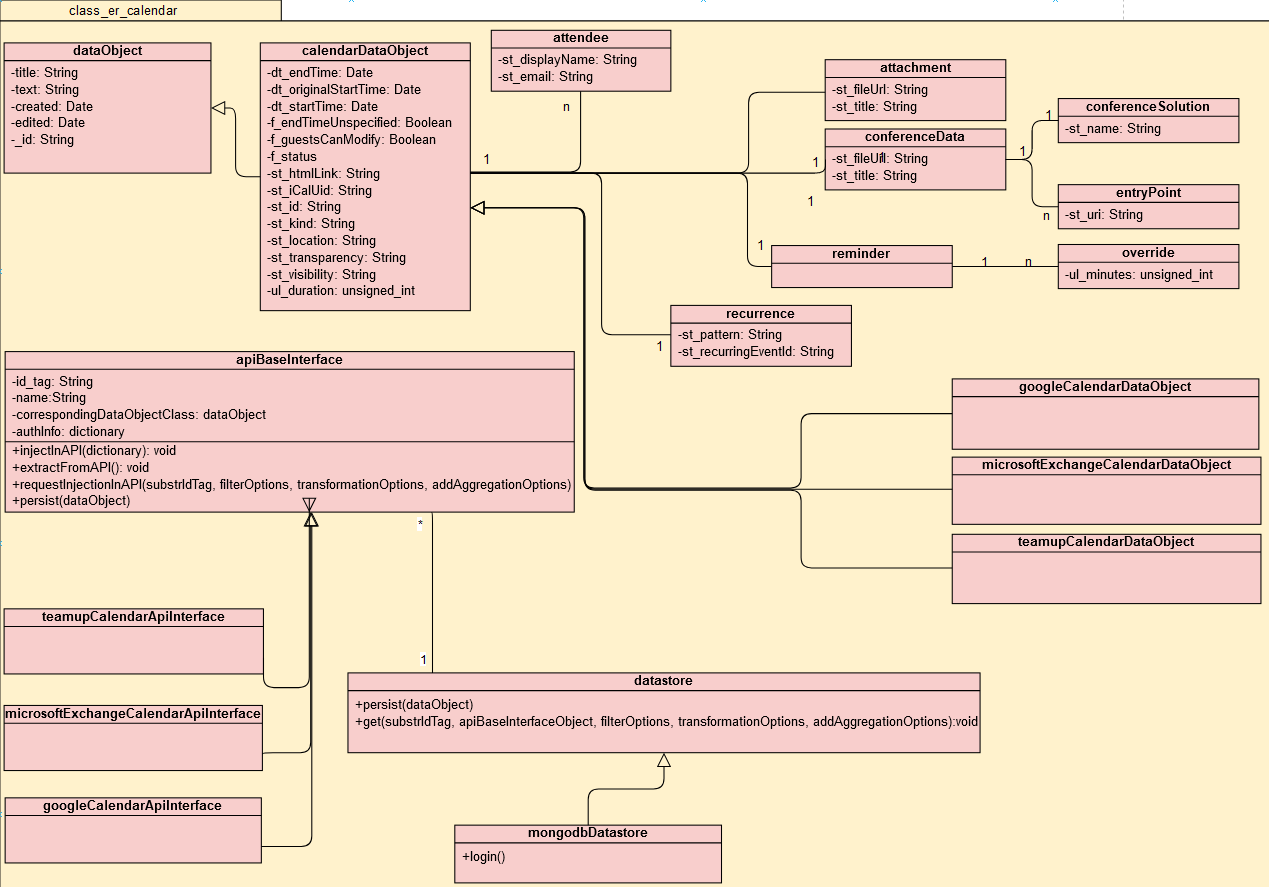
\includegraphics[width=\textwidth]{pics/architecture.png}	
	\caption{Ausschnitt aus der Architektur des Datentransformations- und Verteilungssystems}
	\label{fig:architectur}
\end{figure}

Bevor die Kalender-Services detailliert erläutert werden, ist es sinnvoll, sich einen Überblick über die Architektur des Systems zu verschaffen. Ein Ausschnitt dieser Architektur mit den wichtigsten Komponenten ist in Fig. \ref{fig:architectur} dargestellt. Für dieses Schaubild wurden aus dem Grund der Übersichtlichkeit die Attribute der konkreten Daten-Objekte die von der abstrakten Klasse calendarDataObject erben, und einige Klassen, sowie deren Attribute, die zu der Klasse calendarDataObject gehören, weggelassen.\\
Auf der obersten Ebene befinden sich die abstrakten Klassen apiBaseInterface und dataObject. Erstere definiert die benötigten Methoden um Daten aus einem Service zu lesen und zu schreiben, sowie die Schnittstelle zur konkret verwendeten Datenbank, hier die MongoDB. Bei der Abfrage der API erhält man hierbei eine komplette Liste der Ergebnisse, beim Lesen von der Datenbank wird jedoch ein Iterator für den Datensatz zurückgegeben, wodurch nicht alle Datensätze in den Arbeitsspeicher geladen werden müssen. Daher wird zwischen der Methode requestInjectionInAPI und injectInAPI unterschieden. Die Methode requestInjectionInAPI entspricht einem Aufruf der Datenbank, um alle benötigten Informationen abzufragen. Jeder somit erhaltene Datensatz wird nun innerhalb der Methode einzeln mittels der Methode injectInAPI in den konkreten Service geschrieben. Von dieser Klasse apiBaseInterface erben die konkreten Implementierungen für die verschiedenen Service-Schnittstellen, somit nutzen diese die selbe Datenbank, und müssen die immer gleichen Methoden nicht nochmals implementieren. Einzig die Methoden extractFromAPI und injectInAPI sind individuell für jeden Service und müssen überschrieben werden, sowie die Attribute des apiBaseInterface. Der id\_tag entspricht einer Zusammensetzung aus der Kategorie und dem konkreten ApiInterface-Namen, name entspricht dem Anzeigenamen in der GUI, damit die ApiInterface-Namen dem korrespondierenden Service leichter zugeordnet werden können. Zudem definiert das Attribut authInfo die benötigten Anmeldeinformationen, um sich im Service einloggen zu können, oder spezifische Daten, wie gewünschte Subkalender für die Operation angeben zu können. Um Transformationen korrekt auszuführen, muss zudem bekannt sein, welche Attribute in welchem Service existieren, hierfür kennt das konkrete ApiInterface, das zugehörige konkrete Datenobjekt. Dies würde sich auch über Konventionen für Benennungen lösen lassen, gibt dem Programmierer an dieser Stelle jedoch etwas mehr Freiheiten. \\
Die zweite abstrakte Klasse ist dataObject, diese definiert die Attribute welche über mindestens zwei Kategorien identisch sind und somit für die Transformation von Daten über Kategorien hinweg nötig sind. Die darunterliegende Hierarchie, hier calendarDataObject definiert alle Attribute, die in mehreren Kalenderservices vorhanden sind, somit befinden sich in der untersten Ebene in den konkreten DataObjects nur solche Attribute, die nur im jeweiligen Service vorzufinden sind. Eine Übersicht, welche Attribute der Kalender-Services zu den neu definierten Attribute der Datenobjekte gehören, ist unter dem Link \glqq \url{https://drive.google.com/file/d/1F3JymnclAvFreB0US2ZZT0XHX62KHEG5/view?usp=sharing}\grqq einsehbar. \\
Der Grund für die Wahl von MongoDB ist auf die Flexibilität der Speicherung zurückzuführen. Da alle Services unterschiedliche Daten zurückliefern, macht es Sinn, diese so wie sie sind, als Schlüssel-Wert-Tupel zu speichern, anstatt wie in relationalen Datenbanken üblich, eine einheitliche, hier erzeugte übergroße Struktur mit den Daten zu befüllen, wobei sehr viele Felder leer bleiben würden. \\





 \pagebreak
\section{Google Kalender-Service}
Durch die Bekanntheit und Vielzahl der zur Verfügung stehenden Tools, wird der Google-Kalender von einer sehr großen Bevölkerungsgruppe benutzt. Dieser Universalkalender bietet neben dem Erstellen von Terminen auch viele weitere Möglichkeiten, wie die Verknüpfung der Termine mit mehreren Videokonferenzlösungen, beispielsweise Google-Hangouts, dem Hinzufügen von Dateien, optionalen Gästen oder Ressourcen, um nur wenige zu nennen. Mit über 120 trivialen und komplexen Attributen bietet google zudem sehr viele Optionen, wodurch diese Struktur als Mapping-Grundlage für die weiteren Services dient. Um diese Daten abfragen zu können, muss eine credentials.json-Datei von google angefragt werden, die mit dem Projekt verknüpft wird und als API-Key fungiert. Die Autorisierung erfolgt dann beim Aufruf des Services über den Login im Browser, hierbei wird eine Datei namens token.pickle erstellt, mit dessen Hilfe wäre ein weiterer Login bei künftigen Abfragen nicht mehr notwendig, aus Gründen der Datensicherheit und der erwarteten seltenen Nutzungsrate, ist die Speicherung dieser Datei im Quellcode des googleCalendarApiInterface auskommentiert, kann jedoch, wenn gewünscht, wieder genutzt werden.

\subsection{Erstellen einer Authentifizierungs-Datei}
Um Daten vom Google-Kalender abzufragen oder in diesen zu schreiben, muss zuerst die credentials.json-Datei erstellt werden. Hierzu klickt man auf der Website \url{https://developers.google.com/calendar/quickstart/python}, auf den Button \glqq Enable the Google Calendar API-Key \grqq, wählt einen Projektnamen, den Typ der App, in diesem Fall eine Desktop-App und kann nun, nach dem Klick auf \glqq Create \grqq die Datei zur Authentifizierung herunterladen und in den gewünschten Ordner des Projektes, hier src\textbackslash calendar\textbackslash google, verschieben.

\subsection{Lesende und schreibende Abfragen der Google-API}
Um mit dem Google-Kalender zu interagieren, wird aus den Daten der credentials.json-Datei und den Authentifikationsdaten ein service-Objekt erstellt, mit dem verschiedene Abfragen möglich sind. So können beispielsweise alle Termine abgefragt werden, wobei Serientermine entweder nur aus dem Starttermin mit dem Pattern für die Serie oder dekomprimiert mit allen zugehörigen Terminen enthalten sind, oder es werden Termine in den Google-Kalender mithilfe einer insert-Funktionalität zurückgeschrieben. \\
Bei der GET-Abfrage der Daten aus dem Kalender wird eine Liste von python-Dictionary zurückgegeben, das alle vorhandenen Attribute enthält. Die Anfrage benötigt hierbei die Google-ID des abgefragten Kalenders, als Standard wird der Hauptkalender \glqq primary \grqq verwendet. Zudem kann man nicht nach speziellen Events, wie durch die Angabe eines Start-Datums im von Google gebräuchlichen ISO-8601-Formats, suchen, hierfür ist nur die eindeutige ID des Termins zulässig. \\
Um Termine in den Google-Kalender zu schreiben, werden neben dem konkreten Kalender in den geschrieben werden soll, auch die Informationen über das Start- und Enddatum benötigt. Hierfür wird das konkrete Terminobjekt in ein python-dictionary zurückgeschrieben und der Insert-Funktion \glqq insert(calendarId, body=None, sendNotifications=None, maxAttendees=None, sendUpdates=None, supportsAttachments=None, conferenceDataVersion=None)\grqq{} als \glqq body\grqq{} übergeben. Das Einfügen von Terminen bereitet jedoch ein Problem, wenn bereits zuvor abgefragte Termine, wieder in den google-Kalender zurückgeschrieben werden, da die ID des Termins beim Einfügen ignoriert und neu vergeben wird, somit muss die Entscheidung, ob der Termin bereits existiert, lokal getroffen werden. Hierfür werden von Google einmalig alle Termine abgefragt und die IDs in einer Liste gespeichert. Bevor ein Termin in den Kalender geschrieben wird, muss nun geprüft werden, ob die ID bereits in der Liste vorhandener Termine existiert. Wenn dies der Fall ist, wird der Termin herausgefiltert. Hierbei entsteht nur das Problem, dass Updates der Termine, die beispielsweise über einen weiteren Kalenderdienst vorgenommen wurden, aufgrund der identischen ID, nicht in den Google-Kalender geschrieben werden. \\
Serientermine werden bereits dekomprimiert abgefragt, um die Serienregeln nicht mithilfe eines Tools konvertieren zu müssen, da diese für jeden Service sehr speziell sind und sich stark voneinander unterscheiden. Ein Schreiben von Serienterminen in den Google-Kalender kann mit den in Tab.\ref{tab:google-recurrence} aufgelisteten Parametern innerhalb einer Liste erfolgen \cite{GoogleLLC.13.05.2019}. So ergibt beispielsweise [\grqq{}EXDATE;VALUE=DATE:20150610\grqq{},
\grqq{}RDATE;VALUE=DATE:20150609,20150611\grqq{},
\grqq{}RRULE:FREQ=DAILY;UNTIL=20150628;INTERVAL=3\grqq{}] eine Wiederholung des Termins vom angebenen Startdatum bis zum 28. Juni 2015 im 3-Tages-Rhythmus, wobei der Termin am 10. Juni ausfällt, jedoch am 9. und 11. Juni zusätzlich stattfindet. Anstelle dessen, könne auch hier Serientermine in Form einzelner Termine interpretiert werden, hierbei geht jedoch die Information der Zusammengehörigkeit der Termine verloren.

\begin{table}[h]
	\caption{Beispielhafter Aufbau der Serientermin-Regeln der Google-API}
	\label{tab:google-recurrence}
	\begin{tabularx}{\textwidth}{ | l | X | }
		\hline
		Parameter & Funktion \\ \hline
		EXDATE & Ausgeschlossene Tage \\ 
		RDATE & Zusätzliche Tage \\ 
		RRULE & Regel zur Angabe, wie häufig der Serien-Termin stattfindet \\
		\hline
	\end{tabularx}
\end{table} \pagebreak
\section{Microsoft-Exchange Kalender-Service}
Der Kalender-Dienst von Microsoft ist als Teil des Microsoft-Office Paketes durch den Client Outlook und als Server mit dem Namen Exchange sehr bekannt und sowohl im privaten Bereich als auch in Firmen weit verbreitet. Ein Vorteil des Kalenders ist die Spezialisierung auf die Terminplanung mit der Möglichkeit, Termine als Online-Konferenzen auszuweisen.

\subsection{Login in den Exchange-Service}
Da Microsoft Exchange auf vielen verschiedenen Plattformen installiert werden kann, wird hierbei neben den Login-Daten \glqq Domäne\textbackslash Benutzername\grqq{} und \glqq Passwort\grqq{} auch die Angabe benötigt, unter welcher URL der Exchange-Server erreichbar ist, ein Beispiel hierfür ist: \glqq exchange.othr.de\grqq{}. Daneben ist noch die Angabe der Email-Addresse notwendig, um die Verbindung zum konkreten Account herstellen zu können.
Diese Informationen reichen aus, um alle Daten eines beliebigen Exchange-Kalenders abzufragen und neue Informationen zu ergänzen. 

\subsection{Lesende und schreibende Abfragen der Exchange-API}
Mithilfe der Login-Informationen kann der konkrete Login in einen Account konfiguriert werden, womit die Rechte Termine einzusehen und neue Termine zu erstellen gewährt wird. Aus diesen Daten wird hierbei ein konkretes Account-Objekt erzeugt, mit dessen Hilfe man beispielsweise über die Kalendereinträge, aber auch Emails lokal iterieren kann. \\
Für die Einsicht in die Kalenderdaten gibt es zwei verschiedene Möglichkeiten, einerseits die Methode all(), die alle Termine in ihrer Grundform liefert, Serientermine werden hierbei nicht expandiert. Andererseits kann die Methode view() genutzt werden, diese expandiert Serientermine in die Einzeltermine, womit das zugrundeliegende Pattern nicht manuell interpretiert werden muss. Die hierfür genutzte exchangelib-Bibliothek bietet zudem noch vordefinierte Methoden, um den Datensatz nachzubearbeiten, beispielsweise kann die Reihenfolge an die Erstellreihenfolge der Termine angepasst werden, oder an eine alphabetische Prozessierung über den Titelnamen. Im Gegensatz zum Google-Kalender werden bei der Abfrage des Kalenders alle Subkalender berücksichtigt, könnten jedoch auch weiter über die Namen der Kalender eingeschränkt werden.\\
Das Schreiben von Terminen in einen Kalender gestaltet sich bei Microsoft Exchange Kalendern jedoch als deutlich schwieriger, da auf sehr viele Attribute ein rein lesender Zugriff gestattet ist. So können beispielsweise keine Informationen zum Änderungsdatum, IDs, oder Serienterminen angegeben werden. Dies führt dazu, dass Serientermine nur in Form von Einzelterminen neu eingefügt werden können. Eine Zusammengehörigkeit der Termine lässt sich im Kalender somit nicht mehr erkennen und die Termine lassen sich nicht mehr gemeinsam bearbeiten. Ob ein Eintrag bereits im Exchange-Service vorhanden ist, lässt sich hier jedoch nicht über die IDs erkennen, da diese in einer Abfrage nicht mitgegeben werden. Hierfür wird eine Liste erstellt, die die Sha-256-Werte aus dem Titel des Termins und dem Startdatum enthält. Hiermit sind Vergleiche deutlich performanter, als wenn für jeden existierenden Kalendereintrag mehrere Attribute verglichen werden müssten, zudem ist es sehr unwahrscheinlich, dass zwei Termine auf den selben Wert abgebildet werden. Um einen neuen Kalendereintrag anzulegen, wird ein Calendar-Item-Objekt angelegt, in welchem alle benötigten Attribute angegeben werden. Hierbei können beliebig viele Attribute im Konstruktor angegeben werden. Komplexere Datenstrukturen wie die Teilnehmer und teilweise nicht vorhandene Attribute, wie URLs zu Online-Konferenzlösungen, können auch außerhalb des Konstruktors zugewiesen werden. Um Attribute mit möglichen Standardwerten innerhalb des Konstruktors zuzuweisen, empfiehlt sich hierbei die Verwendung der if-else-expression in python, anstatt des if-else statements, welches innerhalb des Konstruktors nicht verwendet werden kann.
 \pagebreak
\section{Teamup Kalender-Service}
Der Teamup-Kalender ist in der Reihe der hier betrachteten Kalender, das kleinste und unbekannteste Tool, womit dieses die analysierten Kalender gut ergänzt. Der Teamup-Kalender ist spezialisiert auf die Planung von gemeinsamen Terminen, wie Kursen, mit der Möglichkeit, dass sich Teilnehmer bei Erlaubnis selbst zu den Terminen einladen können. 

\subsection{Authentifizierung für einen Teamup-Kalender}
Um auf einen Kalender von Teamup zugreifen zu können, wird nur ein API-Key benötigt, zusammen mit der geheimen Kalender-ID. Der API-Key lässt sich nach dem Einloggen mit einem Teamup-Account auf \url{https://teamup.com/api-keys/request} erstellen, indem man die Email-Addresse, das Unternehmen, und einen optionalen Kommentar angibt und auf \glqq Create API Key \glqq klickt. Der API-Key wird direkt angezeigt und sollte gespeichert werden, da er für jede Abfrage des Kalenders sowie jedes Erzeugen eines neuen Termins benötigt wird. Die geheime Kalender-ID befindet sich bei der Betrachtung eines Kalenders im Browser in der URL. So ist bei dem Kalender auf \url{https://teamup.com/kst496bmane3rty9b7} die geheime ID \glqq kst496bmane3rty9b7\grqq{}. Jeder Benutzer kann mehrere Kalender mit unterschiedlichen Kalender-IDs anlegen, jeder dieser Kalender gliedert sich nochmals in definierbare Unterkalender. Durch die Kenntnis der Kalender-ID ist es jedoch jedem Nutzer möglich, auf jeden ihm bekannten Kalender einer beliebigen anderen Person mittels der API vollen Zugriff zu erhalten.

\subsection{Lesender und schreibender Zugriff auf die Teamup-API}
Bei der Abfrage des Teamup-Kalenders wird die REST-API mittels einer GET-Abfrage \url{https://api.teamup.com/KALENDER-ID/events} zusammen mit einem Teamup-Token, also dem erzeugten API-Key, abgefragt. Hierbei sind Einschränkungen des Zeitraums möglich, indem beides, das Start- und Enddatum mit angegeben werden. Als Antwort erhält man ein JSON-Dokument, das eine Liste mit den gefundenen Kalendereinträge enthält. Eine einfache Fehlerquelle ist hierbei das abgefragte Datum in ISO-8601-Format, da die Zeitzone hierbei nur angegeben wird, wenn diese nicht der Zeitzone UTC entspricht. Hierdurch ergeben sich zwei verschiedene Zeitformate die getrennt voneinander interpretiert werden müssen. \\
Beim Schreiben in den Teamup-Kalender wird eine POST-Anfrage an die Teamup-API geschickt, der Aufbau ist identisch zur GET-Abfrage, nur dass diese um den einzufügenden Termin in Form eines JSON-Dokuments ergänzt wird. Zudem beschränkt die Teamup-API schreibbare Termine auf solche, deren Startzeitpunkt in der Zukunft liegt. Diese Information ist wichtig, um vergangene Termine, beispielsweise vor einem Backup, zu exkludieren. Um doppelte Einträge im Kalender nach einer Schreibaktion zu vermeiden, müssen gesicherte Einträge mit den bereits online vorhandenen Terminen verglichen werden. Da die API keinerlei Informationen über IDs mitteilt, muss auch für diesen Service eine Liste mit Kennzeichen zur Eindeutigkeit erstellt werden. Die Entscheidung lag hierbei ebenso auf einem Sha-256-Mapping aus dem Start-Termin und dem Titel des Eintrags, da es unwahrscheinlich ist, dass zwei unterschiedliche Termine gleich benannt sind und zum selben Termin stattfinden. Ergeben sich aus den Sha-256-Werten für bereits existierende Termine und einem einzufügenden Termin die selben Werte, so wird angenommen, dass dieser bereits im Kalender vorhanden ist, und somit wird dieser nicht mehr neu eingefügt. \pagebreak
\section{Graphische Benutzeroberfläche}
\begin{figure}
	\centering
	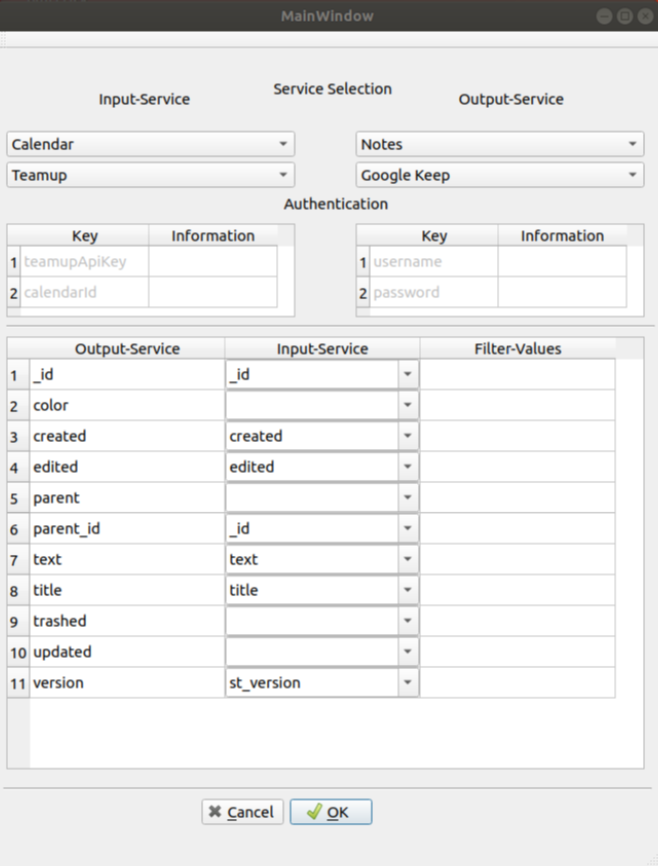
\includegraphics[width=0.6\textwidth]{pics/gui.png}	
	\caption{Graphische Benutzeroberfläche des Systems}
	\label{fig:gui}
\end{figure}
Um den Benutzern den Einstieg in die Anwendung zu erleichtern, wurde eine einfache graphische Benutzeroberfläche mithilfe des QT-Creators erzeugt. Der QT-Creator bietet die Möglichkeit die View-Perspektive der Oberfläche per Drag\&Drop mit den gewünschten Elementen zu befüllen. Hierfür erzeugt der QT-Creator drei Dateien, eine für das Projekt, eine für den aktuellen Bearbeiter des Projekts und eine \glqq .ui\grqq{}-Datei, die den Aufbau der Oberfläche beinhaltet. Mithilfe des pyuic-Tools, dass mit dem PyQt-Paket installiert wird, lässt sich aus der .ui-Datei durch den Befehl \glqq pyuic -o output.py input.uic\grqq{} ein Python-Skript erzeugen, welches die selbe Oberfläche innerhalb einer Klasse, standardmäßig MainWindow, definiert, dies kann jedoch im QT-Creator geändert werden. Ebenso könnte statt dem Python-Skript auch eine C- oder C++-Datei erzeugt werden. \\
Da diese Datei jedoch automatisch generiert ist und nur die View, siehe Abb.\ref{fig:gui}, also keinerlei Logik, enthält, muss diese noch eingepflegt werden. Um die Fortschritte durch ein erneutes Generieren der Oberfläche nicht zu zerstören, erzeugt man eine neue Klasse, die von dieser Oberfläche erbt und implementiert die Logik in der neuen Klasse. \\
Für diese Anwendung soll ein Benutzer die Möglichkeit haben, die Daten von einem beliebigen Service zu extrahieren und in einen neuen Service zu schreiben. Welche Services es gibt, wird mittels Introspection ermittelt, hierbei wird zur Laufzeit unter anderem analysiert, welche Vererbungshierarchien existieren\cite{Chun.2001}. In diesem Projekt entspricht dies, der Findung aller Kindklassen für die Klasse baseApiInterface, nachdem alle zum Projekt gehörigen Python-Skripte importiert wurden. Die möglichen Kategorien und Services ergeben sich über die id\_tags, die in den jeweiligen Service-Klassen definiert werden. \\
Die Login-Informationen, die für einen Service benötigt werden, müssen im Attribut authInfo des Services definiert werden, die möglichen Attribute die in einen Service geschrieben werden können, werden über ein zugehöriges Daten-Objekt definiert und über die Verbindung in der Service-Klasse ausgelesen. Hierbei können in der GUI derzeit nur triviale und keine komplexen Attribute dargestellt werden. Die zugehörigen Attribute des Input-Services werden anhand der Namensähnlichkeit vorbelegt, um diese zu übertragen, hierbei ergeben sich jedoch mehrere mögliche Szenarien. Das erste ist, dass aufgrund der internen, geänderten Namensstruktur keine Werte übereinstimmen, somit müssen alle Mappings der Attribute manuell durchgeführt werden. In der zweiten Variante, wird verglichen, welche Namen der Attribute des Output- oder des Input-Service mit einer genauen Übereinstimmung im jeweils anderen vorkommen, hier erhält man die gemeinsamen Attribute, insofern diese identisch benannt sind. Im dritten Szenario werden beide Richtungen geprüft, ohne genaue Übereinstimmung. Hiermit erhält man eine maximal mögliche Überschneidung, wobei manche Attribute möglicherweise fehlerhaft belegt werden, da die Übereinstimmung zu gering ist. So kann beim Vorhandensein von zehn ID-Feldern jedes mit der gleichen ID vorbelegt sein. Egal welche Variante genutzt wird, ist eine manuelle Überarbeitung notwendig. Durch die Vielzahl an existierenden Attributen, fiel die Wahl jedoch auf die dritte Variante. Statt dem Mapping auf ein Attribut kann auch eine Konstante in das Feld eingetragen werden, zudem ist ein String-Filter setzbar, um die Daten-Objekte anhand gültiger Werte einzuschränken, dass nur diese in einen Service geschrieben werden.

 \pagebreak
\section{MongoDB Datenbank}
Die Datenbank MongoDB bildet die zentrale Instanz der Applikation, in die die Datensätze persistiert werden, und von der die Daten wieder abgefragt werden, um diese in einen Service zu schreiben. Hierbei bietet MongoDB den Vorteil, dass die Daten in einem JSON-ähnlichen Format gespeichert, das auch ähnlich zu den python-Dictionaries aufweist und somit ein hohes Maß an Flexibilität für die Anzahl und Art der Attribute mit sich bringt.\\
Zudem bietet MongoDB die Möglichkeit, Daten die abgefragt werden, direkt über eine Aggregation-Pipeline zu transformieren. Dies erleichtert die Transformation für die einzelnen Services, da hierbei direkt Filter, neue Mappings und Aggregationsmethoden angewandt werden können. Hierfür werden drei Arrays für Parameter definiert: Filteroptionen, zusätzliche Pipeline Schritte und Aggregationsoptionen. \\
Die so erhaltenen Datensätze werden nicht komplett in den Speicher geladen, da durch sehr viele gespeicherte Daten-Objekte auch viel Speicherplatz verbraucht werden kann, daher wird der Iterator verwendet um eine gegebene Funktion auf jedes erhaltene python-Dictionary anzuwenden. Diese Funktionalität wird derzeit genutzt, um jeden Datensatz einzeln in einen Service zu schreiben. Als Folge resultiert ein niedrigerer lokaler Speicherverbrauch, jedoch eine deutlich höhere Anzahl an API-Anfragen.   \pagebreak
\section{Ausblick}
In der derzeitigen Fassung, ist es möglich, Daten über die graphische Benutzeroberfläche von einem Service auszulesen, in die MongoDB zu schreiben, zu filtern, transformieren und in eine weitere API zu schreiben. Hierfür existieren derzeit sechs Services, drei für Kalender und drei für Notizen. In Zukunft ist es vorstellbar, dass hierfür innerhalb der Kategorien viel mehr Services zur Verfügung stehen, und auch Services für neue Kategorien erstellt werden, um weitere Transformationen zu ermöglichen. Zudem bietet auch die GUI einen großen Spielraum, so könnten weitere Filtermöglichkeiten für das Datum oder die Verarbeitung komplexer Attribute ermöglicht werden. Mit einem weiteren Eingabefeld, könnte man es Experten auch gestatten, selbst weitere Stages für die MongoDB Aggregation-Pipeline zu schreiben um viel mächtigere Transformationen zu gewährleisten. Weiter wäre denkbar, einmal getätigte Mappings zwischen Attributen für spätere Aufrufe zu speichern, sodass der Anwender dieses nicht erneut durchführen muss. \\
Wie zu erkennen ist, hat die Anwendung ein sehr großes Potential mit vielen Erweiterungsmöglichkeiten. Sobald genug Services und eine Verbesserung der GUI, im Sinne von einer einfacheren oder mächtigeren Handhabbarkeit, vorhanden sind, ist es denkbar, dass das Tool auch im privaten oder professionellen Bereich zum Zweck von regelmäßigen Datensicherungen oder Datentransformationen genutzt wird. Da es immer mehr verschiedene, spezialisierte Software-as-a-Service-Tools gibt, würde dieses Tool als Schnittstelle einen großen Vorteil bringen, so dass jeder seine Daten für sich wie gewünscht organisieren kann. \pagebreak
%\input{chapters/fazit.tex} \pagebreak
%----------------------------------------------------------------------------------------------------------

%\newpage
% ----------------------------------------------------------------------------------
% Kleine Einführung in LaTeX-Elemente
% ----------------------------------------------------------------------------------
% \section{\LaTeX-Elemente}
% Dieser Abschnitt soll nicht Bestandteil des Projektberichtes sein, sondern beinhaltet lediglich einige
% Informationen über \LaTeX-Distributionen, Editoren und \LaTeX-Elemente, die Ihnen beim Einstieg in das
% \LaTeX-Textsatzsystem helfen sollen.

% \subsection{\LaTeX-Distributionen nach Betriebssystemen}

% \subsubsection{\LaTeX-Distributionen}

% Folgende Haupt-\LaTeX-Distributionen stehen Ihnen zur Verfügung:
% \begin{itemize}
%  \item Windows:\quad \texttt{MiKTeX}\quad Webseite:\quad\url{http://www.miktex.org}
%  \item Linux/Unix:\quad \texttt{TeX Live}\quad Webseite:\quad\url{http://tug.org/texlive/}
%  \item Mac OS:\quad \texttt{MacTeX}\quad Webseite:\quad\url{http://www.tug.org/mactex/}
% \end{itemize}

% \subsubsection{\LaTeX-Editoren}
% Auf folgenden Webseiten können Sie einige hilfreiche \LaTeX-Editoren finden:
% \begin{itemize}
%  \item Windows/Linux/Mac OS: \url{http://www.xm1math.net/texmaker/}
%  \item Windiws: \url{http://www.texniccenter.org/}
%  \item Mac OS: \url{http://pages.uoregon.edu/koch/texshop/}
% \end{itemize}

%Falls bei den oben genannten Editoren kein passender vorhanden war, findet sich auf Wikipedia eine  %Zusammenstellung vieler weiterer \LaTeX-Editoren:\\[1em]
%\hspace*{3cm}\url{https://en.wikipedia.org/wiki/Comparison_of_TeX_editors}


%\subsection{Unterabschnitt}
%Zum Einfügen eines Bildes, siehe Abbildung \ref{fig:reversi01}, wird die
% \textit{minipage}-Umgebung 
%genutzt, da die Bilder so gut positioniert werden können.

%\vspace{1em}
%\begin{minipage}{\linewidth}
%	\centering
%	\includegraphics[width=0.6\linewidth]{pics/gamefield01.png}
%	\captionof{figure}[Spielfeld 01]{Unbespieltes Spielfeld\footnotemark }
%	\label{fig:reversi01}
%\end{minipage}
%\footnotetext{Diesem Spielfeld wurden noch keine Spieler zugewiesen (daher die
% dunklen Spielsteine)}

%Nachdem das Spiel gestartet wurde und beiden Spielphasen durchlaufen wurden, siegt
% schließlich der %Spieler mit der Farbe rot.

%\vspace{1em}
%\begin{minipage}{\linewidth}
%	\centering
%	\includegraphics[width=0.6\linewidth]{pics/gamefield02.png}
%	\captionof{figure}[Spielfeld 02]{Finales Spielfeld\footnotemark }
%	\label{fig:reversi2}
%\end{minipage}
%\footnotetext{Das Spielfeld nach der Zug- und Bombenphase. Spieler rot gewinnt
% eindeutig.}

%\subsection{Tabellen}
%In diesem Abschnitt wird eine Tabelle (siehe Tabelle \ref{tab:beispiel}) dargestellt.

%\vspace{1em}
%\begin{table}[!h]
%	\centering
%	\begin{tabular}{|l|l|l|}
%		\hline
%		\textbf{Name} & \textbf{Name} & \textbf{Name}\\
%		\hline
%		1 & 2 & 3\\
%		\hline
%		4 & 5 & 6\\
%		\hline
%		7 & 8 & 9\\
%		\hline
%	\end{tabular}
%	\caption{Beispieltabelle}
%	\label{tab:beispiel}
%\end{table}


%\subsection{Auflistung}
%Für Auflistungen wird die \textit{enumerate}- oder \textit{itemize}-Umgebung genutzt.
%
%\begin{itemize}
%	\item Nur
%	\item ein
%	\item Beispiel.
%\end{itemize}
%
%\subsection{Listings}
%Zuletzt ein Beispiel für ein Listing, in dem Quellcode eingebunden werden kann, siehe Listing \ref{lst:arduino}.
%
%\vspace{1em}
%\begin{lstlisting}[caption=Arduino Beispielprogramm, label=lst:arduino]
%int ledPin = 13;
%void setup() {
%    pinMode(ledPin, OUTPUT);
%}
%void loop() {
%    digitalWrite(ledPin, HIGH);
%    delay(500);
%    digitalWrite(ledPin, LOW);
%    delay(500);
%}
%\end{lstlisting}
%
%\subsection{Tipps}
%Die Quellen befinden sich in der Datei \textit{quellen.bib}. Eine Buch- und eine Online-Quelle sind beispielhaft eingefügt. [Vgl. \cite{buch}, \cite{online}]
%
%\pagebreak
% ----------------------------------------------------------------------------------------------------------
% Filter fuer Literatur und Quellen definieren
% ----------------------------------------------------------------------------------------------------------

\defbibheading{Literatur}{\section*{Literaturverzeichnis}} 
\defbibheading{Quellen}{\section*{Quellenverzeichnis}} 

\defbibfilter{Literatur}{\not\keyword{online}} 
\defbibfilter{Quellen}{\keyword{online}} 
%\defbibfilter{Literatur}{keyword=trusted} 
%\defbibfilter{Quellen}{keyword=untrusted} 
% ----------------------------------------------------------------------------------------------------------
% Literatur
% ----------------------------------------------------------------------------------------------------------
\addcontentsline{toc}{section}{Literaturverzeichnis}
\addtocontents{toc}{\vspace{-0.5em}}
\lhead{Literaturverzeichnis} 
\rhead{} 
\printbibliography[heading=Literatur,filter=Literatur] 
\pagebreak


% ---------------------------------------------------------------------------------------------------------- 
% Quellen 
% ---------------------------------------------------------------------------------------------------------- 
\addcontentsline{toc}{section}{Quellenverzeichnis}
\addtocontents{toc}{\vspace{-0.5em}}
\lhead{Quellenverzeichnis} 
\rhead{} 
\printbibliography[title = {Quellen}, heading=Quellen,filter=Quellen] 
\pagebreak 

% ----------------------------------------------------------------------------------------------------------
% Anhang
% ----------------------------------------------------------------------------------------------------------
\pagenumbering{Roman}
\setcounter{page}{1}
%\lhead{Anhang \thesection}

%\begin{appendix}
%\section*{Anhang}
%%\phantomsection
%\addcontentsline{toc}{section}{Anhang}
%\addtocontents{toc}{\vspace{-0.5em}}
%
%\end{appendix}

\end{document}
